% Options for packages loaded elsewhere
\PassOptionsToPackage{unicode}{hyperref}
\PassOptionsToPackage{hyphens}{url}
\documentclass[
]{article}
\usepackage{xcolor}
\usepackage[margin=25mm]{geometry}
\usepackage{amsmath,amssymb}
\setcounter{secnumdepth}{-\maxdimen} % remove section numbering
\usepackage{iftex}
\ifPDFTeX
  \usepackage[T1]{fontenc}
  \usepackage[utf8]{inputenc}
  \usepackage{textcomp} % provide euro and other symbols
\else % if luatex or xetex
  \usepackage{unicode-math} % this also loads fontspec
  \defaultfontfeatures{Scale=MatchLowercase}
  \defaultfontfeatures[\rmfamily]{Ligatures=TeX,Scale=1}
\fi
\usepackage{lmodern}
\ifPDFTeX\else
  % xetex/luatex font selection
\fi
% Use upquote if available, for straight quotes in verbatim environments
\IfFileExists{upquote.sty}{\usepackage{upquote}}{}
\IfFileExists{microtype.sty}{% use microtype if available
  \usepackage[]{microtype}
  \UseMicrotypeSet[protrusion]{basicmath} % disable protrusion for tt fonts
}{}
\makeatletter
\@ifundefined{KOMAClassName}{% if non-KOMA class
  \IfFileExists{parskip.sty}{%
    \usepackage{parskip}
  }{% else
    \setlength{\parindent}{0pt}
    \setlength{\parskip}{6pt plus 2pt minus 1pt}}
}{% if KOMA class
  \KOMAoptions{parskip=half}}
\makeatother
\usepackage{color}
\usepackage{fancyvrb}
\newcommand{\VerbBar}{|}
\newcommand{\VERB}{\Verb[commandchars=\\\{\}]}
\DefineVerbatimEnvironment{Highlighting}{Verbatim}{commandchars=\\\{\}}
% Add ',fontsize=\small' for more characters per line
\newenvironment{Shaded}{}{}
\newcommand{\AlertTok}[1]{\textcolor[rgb]{1.00,0.00,0.00}{\textbf{#1}}}
\newcommand{\AnnotationTok}[1]{\textcolor[rgb]{0.38,0.63,0.69}{\textbf{\textit{#1}}}}
\newcommand{\AttributeTok}[1]{\textcolor[rgb]{0.49,0.56,0.16}{#1}}
\newcommand{\BaseNTok}[1]{\textcolor[rgb]{0.25,0.63,0.44}{#1}}
\newcommand{\BuiltInTok}[1]{\textcolor[rgb]{0.00,0.50,0.00}{#1}}
\newcommand{\CharTok}[1]{\textcolor[rgb]{0.25,0.44,0.63}{#1}}
\newcommand{\CommentTok}[1]{\textcolor[rgb]{0.38,0.63,0.69}{\textit{#1}}}
\newcommand{\CommentVarTok}[1]{\textcolor[rgb]{0.38,0.63,0.69}{\textbf{\textit{#1}}}}
\newcommand{\ConstantTok}[1]{\textcolor[rgb]{0.53,0.00,0.00}{#1}}
\newcommand{\ControlFlowTok}[1]{\textcolor[rgb]{0.00,0.44,0.13}{\textbf{#1}}}
\newcommand{\DataTypeTok}[1]{\textcolor[rgb]{0.56,0.13,0.00}{#1}}
\newcommand{\DecValTok}[1]{\textcolor[rgb]{0.25,0.63,0.44}{#1}}
\newcommand{\DocumentationTok}[1]{\textcolor[rgb]{0.73,0.13,0.13}{\textit{#1}}}
\newcommand{\ErrorTok}[1]{\textcolor[rgb]{1.00,0.00,0.00}{\textbf{#1}}}
\newcommand{\ExtensionTok}[1]{#1}
\newcommand{\FloatTok}[1]{\textcolor[rgb]{0.25,0.63,0.44}{#1}}
\newcommand{\FunctionTok}[1]{\textcolor[rgb]{0.02,0.16,0.49}{#1}}
\newcommand{\ImportTok}[1]{\textcolor[rgb]{0.00,0.50,0.00}{\textbf{#1}}}
\newcommand{\InformationTok}[1]{\textcolor[rgb]{0.38,0.63,0.69}{\textbf{\textit{#1}}}}
\newcommand{\KeywordTok}[1]{\textcolor[rgb]{0.00,0.44,0.13}{\textbf{#1}}}
\newcommand{\NormalTok}[1]{#1}
\newcommand{\OperatorTok}[1]{\textcolor[rgb]{0.40,0.40,0.40}{#1}}
\newcommand{\OtherTok}[1]{\textcolor[rgb]{0.00,0.44,0.13}{#1}}
\newcommand{\PreprocessorTok}[1]{\textcolor[rgb]{0.74,0.48,0.00}{#1}}
\newcommand{\RegionMarkerTok}[1]{#1}
\newcommand{\SpecialCharTok}[1]{\textcolor[rgb]{0.25,0.44,0.63}{#1}}
\newcommand{\SpecialStringTok}[1]{\textcolor[rgb]{0.73,0.40,0.53}{#1}}
\newcommand{\StringTok}[1]{\textcolor[rgb]{0.25,0.44,0.63}{#1}}
\newcommand{\VariableTok}[1]{\textcolor[rgb]{0.10,0.09,0.49}{#1}}
\newcommand{\VerbatimStringTok}[1]{\textcolor[rgb]{0.25,0.44,0.63}{#1}}
\newcommand{\WarningTok}[1]{\textcolor[rgb]{0.38,0.63,0.69}{\textbf{\textit{#1}}}}
\usepackage{longtable,booktabs,array}
\newcounter{none} % for unnumbered tables
\usepackage{calc} % for calculating minipage widths
% Correct order of tables after \paragraph or \subparagraph
\usepackage{etoolbox}
\makeatletter
\patchcmd\longtable{\par}{\if@noskipsec\mbox{}\fi\par}{}{}
\makeatother
% Allow footnotes in longtable head/foot
\IfFileExists{footnotehyper.sty}{\usepackage{footnotehyper}}{\usepackage{footnote}}
\makesavenoteenv{longtable}
\usepackage{graphicx}
\makeatletter
\newsavebox\pandoc@box
\newcommand*\pandocbounded[1]{% scales image to fit in text height/width
  \sbox\pandoc@box{#1}%
  \Gscale@div\@tempa{\textheight}{\dimexpr\ht\pandoc@box+\dp\pandoc@box\relax}%
  \Gscale@div\@tempb{\linewidth}{\wd\pandoc@box}%
  \ifdim\@tempb\p@<\@tempa\p@\let\@tempa\@tempb\fi% select the smaller of both
  \ifdim\@tempa\p@<\p@\scalebox{\@tempa}{\usebox\pandoc@box}%
  \else\usebox{\pandoc@box}%
  \fi%
}
% Set default figure placement to htbp
\def\fps@figure{htbp}
\makeatother
\setlength{\emergencystretch}{3em} % prevent overfull lines
\providecommand{\tightlist}{%
  \setlength{\itemsep}{0pt}\setlength{\parskip}{0pt}}
\usepackage{bookmark}
\IfFileExists{xurl.sty}{\usepackage{xurl}}{} % add URL line breaks if available
\urlstyle{same}
\hypersetup{
  hidelinks,
  pdfcreator={LaTeX via pandoc}}

\author{}
\date{}

\begin{document}

\section{Preliminary Summary of Acceleration-Basis and Localization
Exchange in Exchange-Interference Scattering-Matrix Fermion-Like
Collisions
v1}\label{preliminary-summary-of-acceleration-basis-and-localization-exchange-in-exchange-interference-scattering-matrix-fermion-like-collisions-v1}

\textbf{Subtitle:} Localization redistribution in one-sided
high-harmonic recursive scattering while preserving acceleration-like
readout\\
\textbf{Date:} 2026-07-13\\
\textbf{Author:} Noriaki Kihara\\
\textbf{Position:} Wave Information Readout series, preliminary
experiment summary\\
\textbf{Version DOI:} 10.5281/zenodo.21333768\\
\textbf{Concept DOI:} 10.5281/zenodo.21333766

\begin{center}\rule{0.5\linewidth}{0.5pt}\end{center}

\subsection{Abstract}\label{abstract}

This paper summarizes preliminary experiments in which the
exchange-interference scattering-matrix version of the fermion-like
recoil map established in the V2 series is placed on the basis of the AB
two-body acceleration-like readout.

The experiments cover the low odd-harmonic bottom, readout-stop control,
removal of name hair, one-sided high-harmonic conditions, recursive
scattering, and reflection-rate sweeps.

The acceleration V2 basis was preserved. The odd-harmonic bottom was
\texttt{N=1}, both with and without name hair. In the readout-stop
control, the difference in the localization index \texttt{L} was
\texttt{0.0}.

When the one-sided high-harmonic condition \texttt{N\_A=1},
\texttt{N\_B=63} was inserted into recursive scattering, the difference
between low-order and high-order waveforms was preserved at the
complete-transmission endpoint \texttt{R=0} and the complete-reflection
endpoint \texttt{R=1}. In contrast, for intermediate scattering
\texttt{0\textless{}R\textless{}1}, the localization index \texttt{L}
and the effective harmonic order \texttt{N\_eff} were exchanged
periodically.

In the reflection-rate sweep, \texttt{R=0.70} gave the minimum
\texttt{L} difference, \texttt{2.48676e-05}, with \texttt{N\_eff}
difference \texttt{0.153386}. This is recorded as a recursive point at
which the localization indices and effective harmonic orders of the two
channels become close under the one-sided high-harmonic condition.

Within the range of this experiment, stationary convergence was not
observed. The observed behavior was periodic localization exchange
generated by a two-channel scattering matrix without a dissipative term.

\begin{center}\rule{0.5\linewidth}{0.5pt}\end{center}

\subsection{1. Purpose of the
Experiment}\label{purpose-of-the-experiment}

The purpose of this experiment is the following:

\begin{Shaded}
\begin{Highlighting}[]
\NormalTok{To read whether a one{-}sided high harmonic moves into the localization readout}
\NormalTok{of the other channel on a fermion{-}like recoil map that preserves acceleration{-}like readout.}
\end{Highlighting}
\end{Shaded}

Here, localization is not the position of a particle placed in an
external space. It is a quantity read from the \texttt{chi}-direction
density, harmonic distribution, effective harmonic order, and
localization index constructed inside the closed phase system.

The readout targets are the following quantities on the
scattering-matrix outgoing channels:

\begin{Shaded}
\begin{Highlighting}[]
\NormalTok{L}
\NormalTok{N\_eff}
\NormalTok{rho\_chi}
\NormalTok{expected\_origin\_A}
\NormalTok{expected\_origin\_B}
\end{Highlighting}
\end{Shaded}

The experiment records how these quantities are redistributed on the
outgoing channels of the scattering matrix.

\begin{center}\rule{0.5\linewidth}{0.5pt}\end{center}

\subsection{2. Basis Map}\label{basis-map}

From the exchange-interference phase \texttt{Delta\_F}, define the
transmission amplitude \texttt{t} and reflection amplitude \texttt{r}:

\begin{Shaded}
\begin{Highlighting}[]
\NormalTok{t\_\textbackslash{}Delta}
\NormalTok{=}
\NormalTok{e\^{}\{i\textbackslash{}Delta\_F/2\}}
\NormalTok{\textbackslash{}cos\textbackslash{}frac\{\textbackslash{}Delta\_F\}\{2\}}
\end{Highlighting}
\end{Shaded}

\begin{Shaded}
\begin{Highlighting}[]
\NormalTok{r\_\textbackslash{}Delta}
\NormalTok{=}
\NormalTok{{-}i e\^{}\{i\textbackslash{}Delta\_F/2\}}
\NormalTok{\textbackslash{}sin\textbackslash{}frac\{\textbackslash{}Delta\_F\}\{2\}}
\end{Highlighting}
\end{Shaded}

The reflection and transmission rates are read as

\begin{Shaded}
\begin{Highlighting}[]
\NormalTok{R=|r\_\textbackslash{}Delta|\^{}2}
\end{Highlighting}
\end{Shaded}

\begin{Shaded}
\begin{Highlighting}[]
\NormalTok{T=|t\_\textbackslash{}Delta|\^{}2.}
\end{Highlighting}
\end{Shaded}

The two-channel output in this experiment is

\begin{Shaded}
\begin{Highlighting}[]
\NormalTok{minus\_out = r A\_ref + t B\_trans}
\NormalTok{plus\_out  = t A\_trans + r B\_ref}
\end{Highlighting}
\end{Shaded}

In the recursive experiment, the outgoing channels are passed to the
next input:

\begin{Shaded}
\begin{Highlighting}[]
\NormalTok{A\_\{k+1\}}
\NormalTok{=}
\NormalTok{\textbackslash{}operatorname\{norm\}}
\NormalTok{\textbackslash{}left(}
\NormalTok{r A\_k + t B\_k}
\NormalTok{\textbackslash{}right)}
\end{Highlighting}
\end{Shaded}

\begin{Shaded}
\begin{Highlighting}[]
\NormalTok{B\_\{k+1\}}
\NormalTok{=}
\NormalTok{\textbackslash{}operatorname\{norm\}}
\NormalTok{\textbackslash{}left(}
\NormalTok{t A\_k + r B\_k}
\NormalTok{\textbackslash{}right).}
\end{Highlighting}
\end{Shaded}

This recursive map contains no dissipative term.

\begin{center}\rule{0.5\linewidth}{0.5pt}\end{center}

\subsection{3. Acceleration V2 Basis}\label{acceleration-v2-basis}

This experiment uses the AB two-body acceleration V2 result as its
basis.

{\def\LTcaptype{none} % do not increment counter
\begin{longtable}[]{@{}lr@{}}
\toprule\noalign{}
Quantity & Value \\
\midrule\noalign{}
\endhead
\bottomrule\noalign{}
\endlastfoot
fermionic\_reflection\_rate & \texttt{1.0} \\
fermionic\_transmission\_rate & \texttt{3.749399456654644e-33} \\
fermionic\_q\_out\_factor & \texttt{-1.0} \\
max\_Q\_closed\_abs & \texttt{0.0} \\
label\_free\_pass\_vs\_fermionic\_match\_all\_cases & \texttt{true} \\
fermionic\_regular\_cell\_harmonic\_consistent\_nonstrong\_modes &
\texttt{true} \\
fermionic\_c1\_area\_sweep\_detected\_all\_cases & \texttt{true} \\
\end{longtable}
}

Therefore, the scattering-matrix version of the fermion-like recoil map
preserves the basis of the acceleration-like readout.

\begin{center}\rule{0.5\linewidth}{0.5pt}\end{center}

\subsection{4. Low Odd-Harmonic Bottom}\label{low-odd-harmonic-bottom}

Under complete reflection \texttt{Delta\_F=pi}, the odd-harmonic order
\texttt{N} was lowered.

{\def\LTcaptype{none} % do not increment counter
\begin{longtable}[]{@{}lr@{}}
\toprule\noalign{}
Condition & Bottom \\
\midrule\noalign{}
\endhead
\bottomrule\noalign{}
\endlastfoot
With name hair & \texttt{N=1} \\
Without name hair & \texttt{N=1} \\
\end{longtable}
}

Even at \texttt{N=1}, the direction readout and internal readout did not
break down.

Representative values are as follows:

{\def\LTcaptype{none} % do not increment counter
\begin{longtable}[]{@{}
  >{\raggedleft\arraybackslash}p{(\linewidth - 14\tabcolsep) * \real{0.1290}}
  >{\raggedright\arraybackslash}p{(\linewidth - 14\tabcolsep) * \real{0.0968}}
  >{\raggedleft\arraybackslash}p{(\linewidth - 14\tabcolsep) * \real{0.1290}}
  >{\raggedleft\arraybackslash}p{(\linewidth - 14\tabcolsep) * \real{0.1290}}
  >{\raggedleft\arraybackslash}p{(\linewidth - 14\tabcolsep) * \real{0.1290}}
  >{\raggedleft\arraybackslash}p{(\linewidth - 14\tabcolsep) * \real{0.1290}}
  >{\raggedleft\arraybackslash}p{(\linewidth - 14\tabcolsep) * \real{0.1290}}
  >{\raggedleft\arraybackslash}p{(\linewidth - 14\tabcolsep) * \real{0.1290}}@{}}
\toprule\noalign{}
\begin{minipage}[b]{\linewidth}\raggedleft
N
\end{minipage} & \begin{minipage}[b]{\linewidth}\raggedright
hair
\end{minipage} & \begin{minipage}[b]{\linewidth}\raggedleft
p\_chi
\end{minipage} & \begin{minipage}[b]{\linewidth}\raggedleft
d\_q
\end{minipage} & \begin{minipage}[b]{\linewidth}\raggedleft
chi center-cell mass
\end{minipage} & \begin{minipage}[b]{\linewidth}\raggedleft
chi peak contrast
\end{minipage} & \begin{minipage}[b]{\linewidth}\raggedleft
L
\end{minipage} & \begin{minipage}[b]{\linewidth}\raggedleft
total name hair
\end{minipage} \\
\midrule\noalign{}
\endhead
\bottomrule\noalign{}
\endlastfoot
1 & true & \texttt{-1} & \texttt{4.44089e-16} & \texttt{0.5} &
\texttt{2} & \texttt{0.000183105} & \texttt{1} \\
1 & false & \texttt{-1} & \texttt{8.88178e-16} & \texttt{0.5} &
\texttt{2} & \texttt{0.000183105} & \texttt{0} \\
\end{longtable}
}

From this result, the readout bottom under the present experimental
conditions is read as \texttt{N=1}.

Under the present experimental conditions, increasing the odd-harmonic
order mainly appeared as a sharpening of the \texttt{chi}-direction
density, rather than as the presence or absence of information.

\begin{figure}
\centering
\pandocbounded{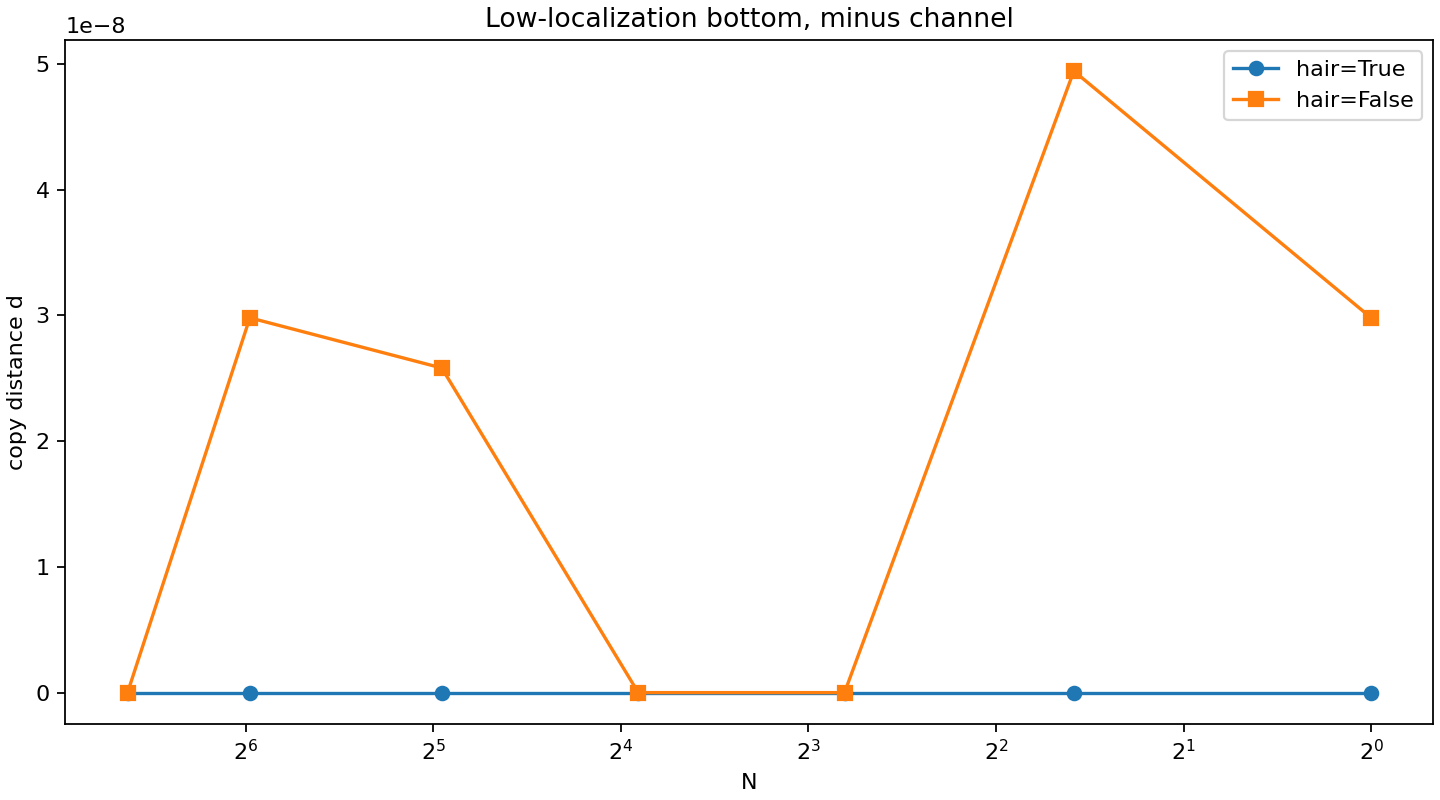
\includegraphics[keepaspectratio,alt={low N}]{exchange_scattering_matrix_fermionic_localization_transfer_preliminary_result_v1/exchange_scattering_matrix_low_n_bottom_v1.png}}
\caption{low N}
\end{figure}

\begin{center}\rule{0.5\linewidth}{0.5pt}\end{center}

\subsection{5. One-Sided High-Harmonic
Condition}\label{one-sided-high-harmonic-condition}

Using the bottom \texttt{N\_A=1} as the reference, the experiment
examined a condition in which only one side has high harmonics.

The representative condition is

\begin{Shaded}
\begin{Highlighting}[]
\NormalTok{N\_A = 1}
\NormalTok{N\_B = 63}
\end{Highlighting}
\end{Shaded}

In one-step scattering with \texttt{R=0.55}, \texttt{T=0.45}, the
outgoing channels retained the allocation of A-origin and B-origin
components.

{\def\LTcaptype{none} % do not increment counter
\begin{longtable}[]{@{}
  >{\raggedright\arraybackslash}p{(\linewidth - 12\tabcolsep) * \real{0.1111}}
  >{\raggedleft\arraybackslash}p{(\linewidth - 12\tabcolsep) * \real{0.1481}}
  >{\raggedleft\arraybackslash}p{(\linewidth - 12\tabcolsep) * \real{0.1481}}
  >{\raggedleft\arraybackslash}p{(\linewidth - 12\tabcolsep) * \real{0.1481}}
  >{\raggedleft\arraybackslash}p{(\linewidth - 12\tabcolsep) * \real{0.1481}}
  >{\raggedleft\arraybackslash}p{(\linewidth - 12\tabcolsep) * \real{0.1481}}
  >{\raggedleft\arraybackslash}p{(\linewidth - 12\tabcolsep) * \real{0.1481}}@{}}
\toprule\noalign{}
\begin{minipage}[b]{\linewidth}\raggedright
channel
\end{minipage} & \begin{minipage}[b]{\linewidth}\raggedleft
R
\end{minipage} & \begin{minipage}[b]{\linewidth}\raggedleft
T
\end{minipage} & \begin{minipage}[b]{\linewidth}\raggedleft
N\_eff
\end{minipage} & \begin{minipage}[b]{\linewidth}\raggedleft
L
\end{minipage} & \begin{minipage}[b]{\linewidth}\raggedleft
origin\_A
\end{minipage} & \begin{minipage}[b]{\linewidth}\raggedleft
origin\_B
\end{minipage} \\
\midrule\noalign{}
\endhead
\bottomrule\noalign{}
\endlastfoot
minus\_out & \texttt{0.55} & \texttt{0.45} & \texttt{14.95} &
\texttt{0.00135002} & \texttt{0.55} & \texttt{0.45} \\
plus\_out & \texttt{0.55} & \texttt{0.45} & \texttt{18.05} &
\texttt{0.0018526} & \texttt{0.45} & \texttt{0.55} \\
\end{longtable}
}

At the one-step scattering stage, the one-sided high harmonic is
allocated to the outgoing channels.

\begin{figure}
\centering
\pandocbounded{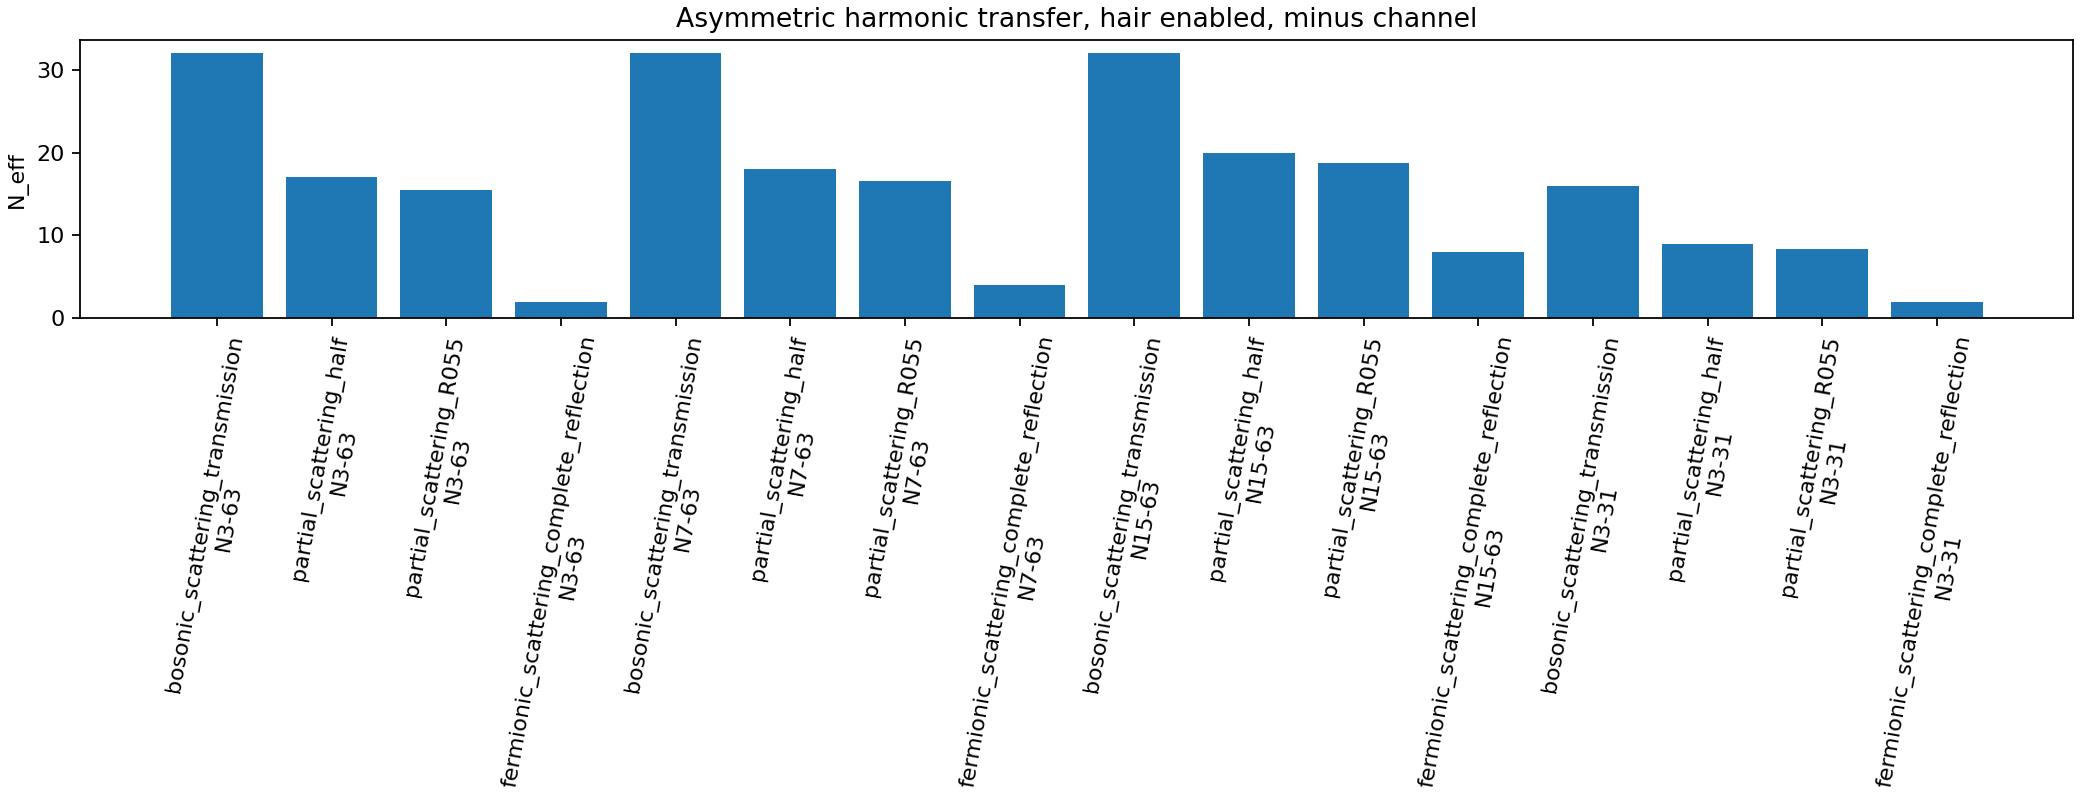
\includegraphics[keepaspectratio,alt={one side high harmonic}]{exchange_scattering_matrix_fermionic_localization_transfer_preliminary_result_v1/exchange_scattering_matrix_one_side_high_harmonic_v1.png}}
\caption{one side high harmonic}
\end{figure}

\begin{center}\rule{0.5\linewidth}{0.5pt}\end{center}

\subsection{6. Recursive One-Sided High
Harmonic}\label{recursive-one-sided-high-harmonic}

The outgoing channels were passed to the next input, and recursive
scattering was performed up to 128 collisions.

The representative result for \texttt{R=0.55}, \texttt{T=0.45} is as
follows:

{\def\LTcaptype{none} % do not increment counter
\begin{longtable}[]{@{}rrrrr@{}}
\toprule\noalign{}
collision & A: L & A: N\_eff & B: L & B: N\_eff \\
\midrule\noalign{}
\endhead
\bottomrule\noalign{}
\endlastfoot
0 & \texttt{0.000183105} & \texttt{1} & \texttt{0.00520897} &
\texttt{32} \\
16 & \texttt{0.00167148} & \texttt{16.9941} & \texttt{0.00151127} &
\texttt{16.0059} \\
32 & \texttt{0.00519937} & \texttt{31.9685} & \texttt{0.000183722} &
\texttt{1.0315} \\
64 & \texttt{0.000185626} & \texttt{1.12587} & \texttt{0.00517067} &
\texttt{31.8741} \\
128 & \texttt{0.000194012} & \texttt{1.50145} & \texttt{0.00505728} &
\texttt{31.4985} \\
\end{longtable}
}

The localization index and effective harmonic order did not converge to
a stationary value.

The recursive map periodically exchanged the low-order side and the
high-order side.

\begin{figure}
\centering
\pandocbounded{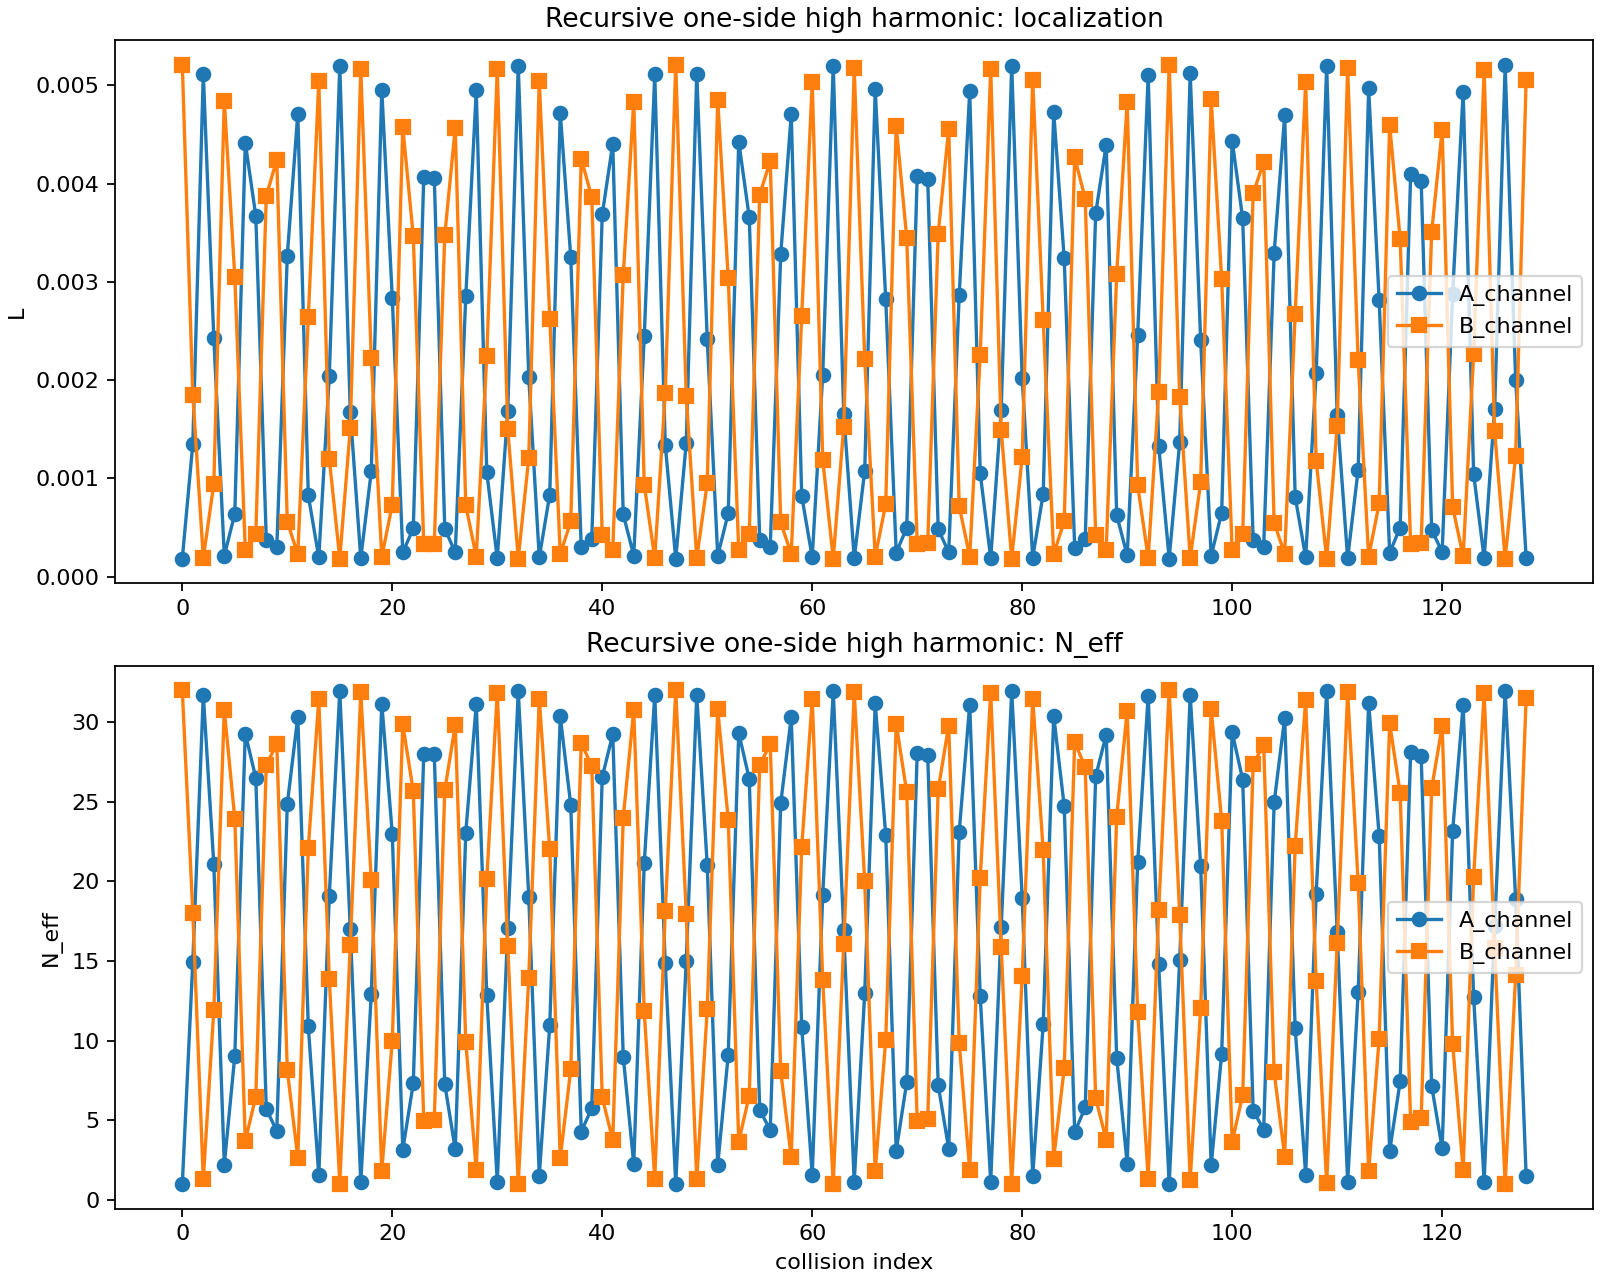
\includegraphics[keepaspectratio,alt={recursive localization transfer}]{exchange_scattering_matrix_fermionic_localization_transfer_preliminary_result_v1/exchange_scattering_matrix_recursive_localization_transfer_v1.png}}
\caption{recursive localization transfer}
\end{figure}

\begin{center}\rule{0.5\linewidth}{0.5pt}\end{center}

\subsection{7. Reflection-Rate Sweep}\label{reflection-rate-sweep}

The reflection rate \texttt{R} was swept under the condition
\texttt{N\_A=1}, \texttt{N\_B=63}.

{\def\LTcaptype{none} % do not increment counter
\begin{longtable}[]{@{}
  >{\raggedleft\arraybackslash}p{(\linewidth - 8\tabcolsep) * \real{0.2000}}
  >{\raggedleft\arraybackslash}p{(\linewidth - 8\tabcolsep) * \real{0.2000}}
  >{\raggedleft\arraybackslash}p{(\linewidth - 8\tabcolsep) * \real{0.2000}}
  >{\raggedleft\arraybackslash}p{(\linewidth - 8\tabcolsep) * \real{0.2000}}
  >{\raggedleft\arraybackslash}p{(\linewidth - 8\tabcolsep) * \real{0.2000}}@{}}
\toprule\noalign{}
\begin{minipage}[b]{\linewidth}\raggedleft
R
\end{minipage} & \begin{minipage}[b]{\linewidth}\raggedleft
T
\end{minipage} & \begin{minipage}[b]{\linewidth}\raggedleft
minimum L difference
\end{minipage} & \begin{minipage}[b]{\linewidth}\raggedleft
collision at minimum L difference
\end{minipage} & \begin{minipage}[b]{\linewidth}\raggedleft
N\_eff difference at minimum L difference
\end{minipage} \\
\midrule\noalign{}
\endhead
\bottomrule\noalign{}
\endlastfoot
0 & 1 & \texttt{0.00502586} & \texttt{1} & \texttt{31} \\
0.51 & 0.49 & \texttt{5.37371e-05} & \texttt{78} & \texttt{0.331455} \\
0.55 & 0.45 & \texttt{0.000114791} & \texttt{110} & \texttt{0.708042} \\
0.6 & 0.4 & \texttt{0.000185909} & \texttt{125} & \texttt{1.1467} \\
0.7 & 0.3 & \texttt{2.48676e-05} & \texttt{42} & \texttt{0.153386} \\
0.9 & 0.1 & \texttt{8.21216e-05} & \texttt{61} & \texttt{0.506534} \\
1 & \texttt{3.7494e-33} & \texttt{0.00502586} & \texttt{126} &
\texttt{31} \\
\end{longtable}
}

At the complete-transmission endpoint \texttt{R=0}, the difference
between the low-order waveform and the high-order waveform was
preserved.

At the complete-reflection endpoint \texttt{R=1}, the difference between
the low-order waveform and the high-order waveform was also preserved.

For intermediate scattering \texttt{0\textless{}R\textless{}1},
recursive points appeared at which the differences in \texttt{L} and
\texttt{N\_eff} became small.

In this sweep, \texttt{R=0.70} gave the minimum \texttt{L} difference.

\begin{figure}
\centering
\pandocbounded{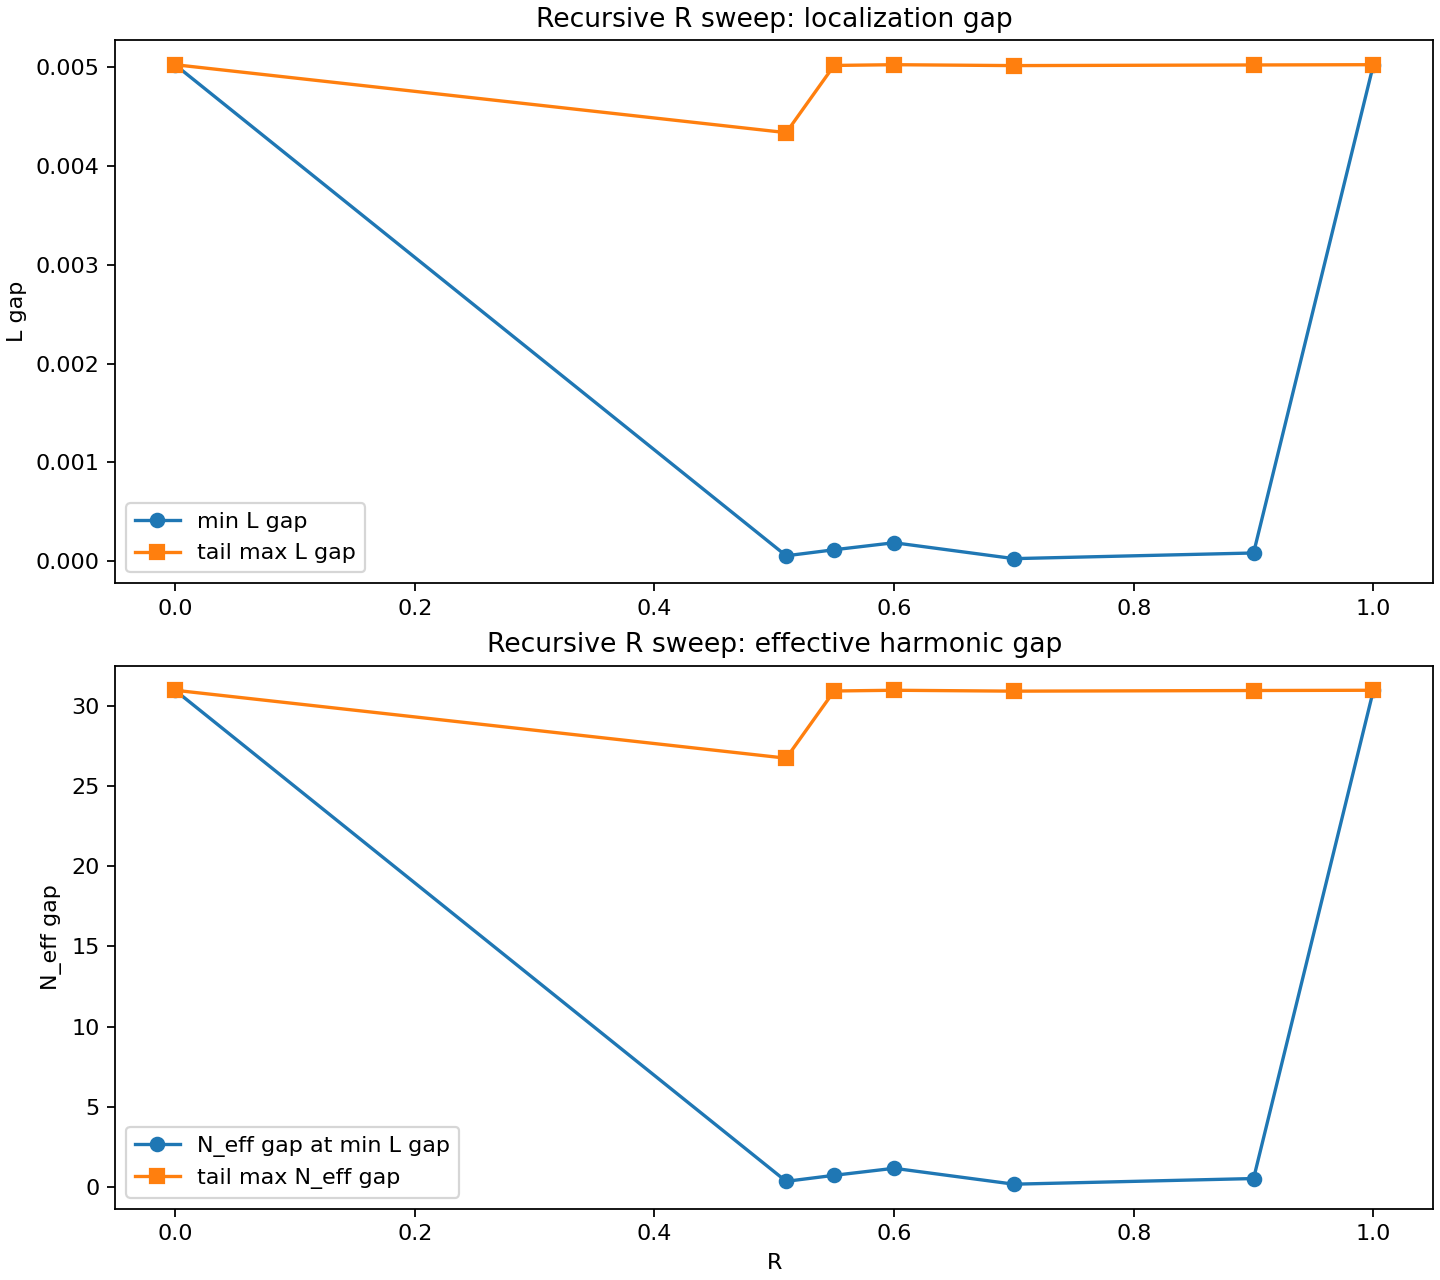
\includegraphics[keepaspectratio,alt={recursive R sweep}]{exchange_scattering_matrix_fermionic_localization_transfer_preliminary_result_v1/exchange_scattering_matrix_recursive_R_sweep_v1.png}}
\caption{recursive R sweep}
\end{figure}

\begin{center}\rule{0.5\linewidth}{0.5pt}\end{center}

\subsection{8. Waveform Localization
Snapshots}\label{waveform-localization-snapshots}

The reduced density in the \texttt{chi} direction is read as

\begin{Shaded}
\begin{Highlighting}[]
\NormalTok{\textbackslash{}rho\_\textbackslash{}chi}
\NormalTok{=}
\NormalTok{\textbackslash{}sum\_\textbackslash{}eta |\textbackslash{}psi(\textbackslash{}chi,\textbackslash{}eta)|\^{}2.}
\end{Highlighting}
\end{Shaded}

In the figures, each line is amplitude-normalized so that its maximum
value is \texttt{1}.

The figure compares the complete-transmission endpoint \texttt{R=0}, the
intermediate scattering case \texttt{R=0.70}, and the
complete-reflection endpoint \texttt{R=1}.

At \texttt{R=0}, A and B are exchanged on the fixed channels. However,
the difference between the low-order waveform and the high-order
waveform itself is preserved.

At \texttt{R=1}, the difference between the low-order waveform and the
high-order waveform is preserved even on the fixed channels.

At \texttt{R=0.70}, the localization indices of the two channels become
close at collision \texttt{42}.

{\def\LTcaptype{none} % do not increment counter
\begin{longtable}[]{@{}
  >{\raggedright\arraybackslash}p{(\linewidth - 10\tabcolsep) * \real{0.1304}}
  >{\raggedleft\arraybackslash}p{(\linewidth - 10\tabcolsep) * \real{0.1739}}
  >{\raggedleft\arraybackslash}p{(\linewidth - 10\tabcolsep) * \real{0.1739}}
  >{\raggedleft\arraybackslash}p{(\linewidth - 10\tabcolsep) * \real{0.1739}}
  >{\raggedleft\arraybackslash}p{(\linewidth - 10\tabcolsep) * \real{0.1739}}
  >{\raggedleft\arraybackslash}p{(\linewidth - 10\tabcolsep) * \real{0.1739}}@{}}
\toprule\noalign{}
\begin{minipage}[b]{\linewidth}\raggedright
Condition
\end{minipage} & \begin{minipage}[b]{\linewidth}\raggedleft
collision
\end{minipage} & \begin{minipage}[b]{\linewidth}\raggedleft
A: L
\end{minipage} & \begin{minipage}[b]{\linewidth}\raggedleft
A: N\_eff
\end{minipage} & \begin{minipage}[b]{\linewidth}\raggedleft
B: L
\end{minipage} & \begin{minipage}[b]{\linewidth}\raggedleft
B: N\_eff
\end{minipage} \\
\midrule\noalign{}
\endhead
\bottomrule\noalign{}
\endlastfoot
R=0 & 0 & \texttt{0.000183105} & \texttt{1} & \texttt{0.00520897} &
\texttt{32} \\
R=0 & 1 & \texttt{0.00520897} & \texttt{32} & \texttt{0.000183105} &
\texttt{1} \\
R=0.70 & 0 & \texttt{0.000183105} & \texttt{1} & \texttt{0.00520897} &
\texttt{32} \\
R=0.70 & 42 & \texttt{0.0016027127797281328} &
\texttt{16.576692758470564} & \texttt{0.0015778452089655066} &
\texttt{16.42330724152941} \\
R=1 & 0 & \texttt{0.000183105} & \texttt{1} & \texttt{0.00520897} &
\texttt{32} \\
R=1 & 1 & \texttt{0.000183105} & \texttt{1} & \texttt{0.00520897} &
\texttt{32} \\
\end{longtable}
}

This figure records, as amplitude-normalized density waveforms, that
localization redistribution appears in intermediate scattering and not
at the endpoints.

\begin{figure}
\centering
\pandocbounded{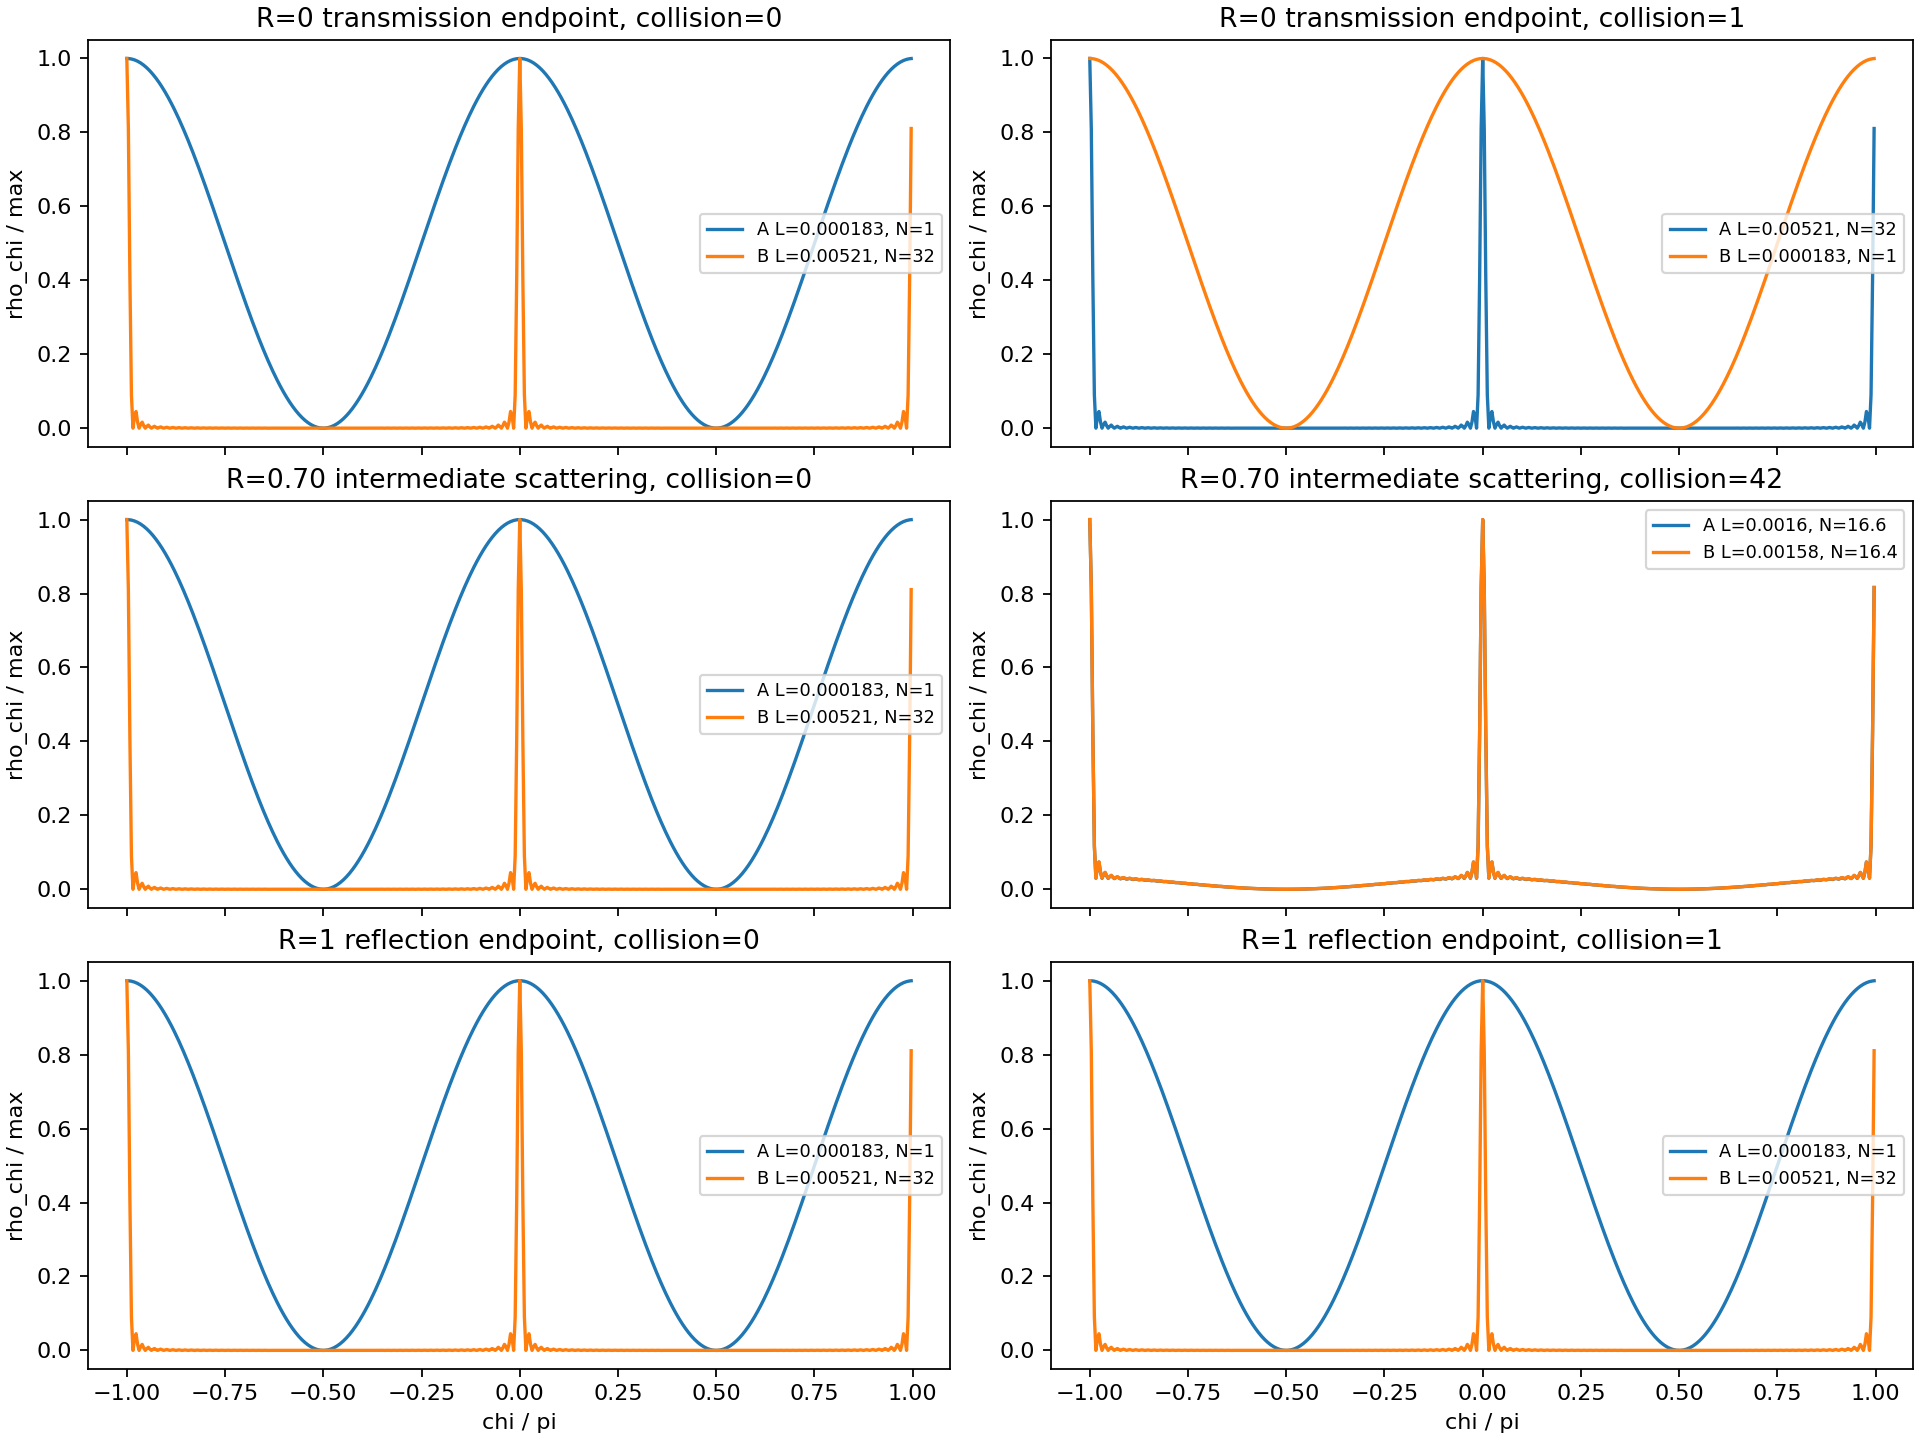
\includegraphics[keepaspectratio,alt={waveform localization snapshots}]{exchange_scattering_matrix_fermionic_localization_transfer_preliminary_result_v1/exchange_scattering_matrix_waveform_localization_snapshots_v1.png}}
\caption{waveform localization snapshots}
\end{figure}

\subsubsection{8.1 Localization-Exchange Process at
R=0.70}\label{localization-exchange-process-at-r0.70}

For \texttt{R=0.70}, the figure shows \texttt{rho\_chi\ /\ max} at
collision counts \texttt{0,1,2,3,5,10,20,42}.

At \texttt{collision=42}, \texttt{L} and \texttt{N\_eff} for A/B are
close, and the localization indices of the two waveforms become close.

The process read from the figure is not monotonic localization, but an
exchange oscillation of localization.

{\def\LTcaptype{none} % do not increment counter
\begin{longtable}[]{@{}
  >{\raggedleft\arraybackslash}p{(\linewidth - 2\tabcolsep) * \real{0.5714}}
  >{\raggedright\arraybackslash}p{(\linewidth - 2\tabcolsep) * \real{0.4286}}@{}}
\toprule\noalign{}
\begin{minipage}[b]{\linewidth}\raggedleft
collision
\end{minipage} & \begin{minipage}[b]{\linewidth}\raggedright
State read from the figure
\end{minipage} \\
\midrule\noalign{}
\endhead
\bottomrule\noalign{}
\endlastfoot
0 & A starts as a low-order base waveform, while B starts as a
high-order localized waveform. \\
1 & A receives high-order components, and the waveform peak of A
sharpens. \\
2,3 & A moves toward the high-localization side, while B moves toward a
dull shape close to the low-order base waveform. \\
5,10 & A becomes dull again, and the high-localization shape returns to
the B side. \\
42 & The effective orders of A/B become close, \texttt{16.6} and
\texttt{16.4}, and their localization indices become close. \\
\end{longtable}
}

From this figure, the one-sided high-localization shape is not simply
averaged away in one step. Instead, it is read as moving back and forth
between A and B through the recursive action of intermediate scattering.
Near \texttt{collision=42}, the effective order is lower than the
initial B value \texttt{N\_eff=32}, while the amplitude-normalized
waveform still retains a sharp shape that is not only the low-order base
wave.

\begin{figure}
\centering
\pandocbounded{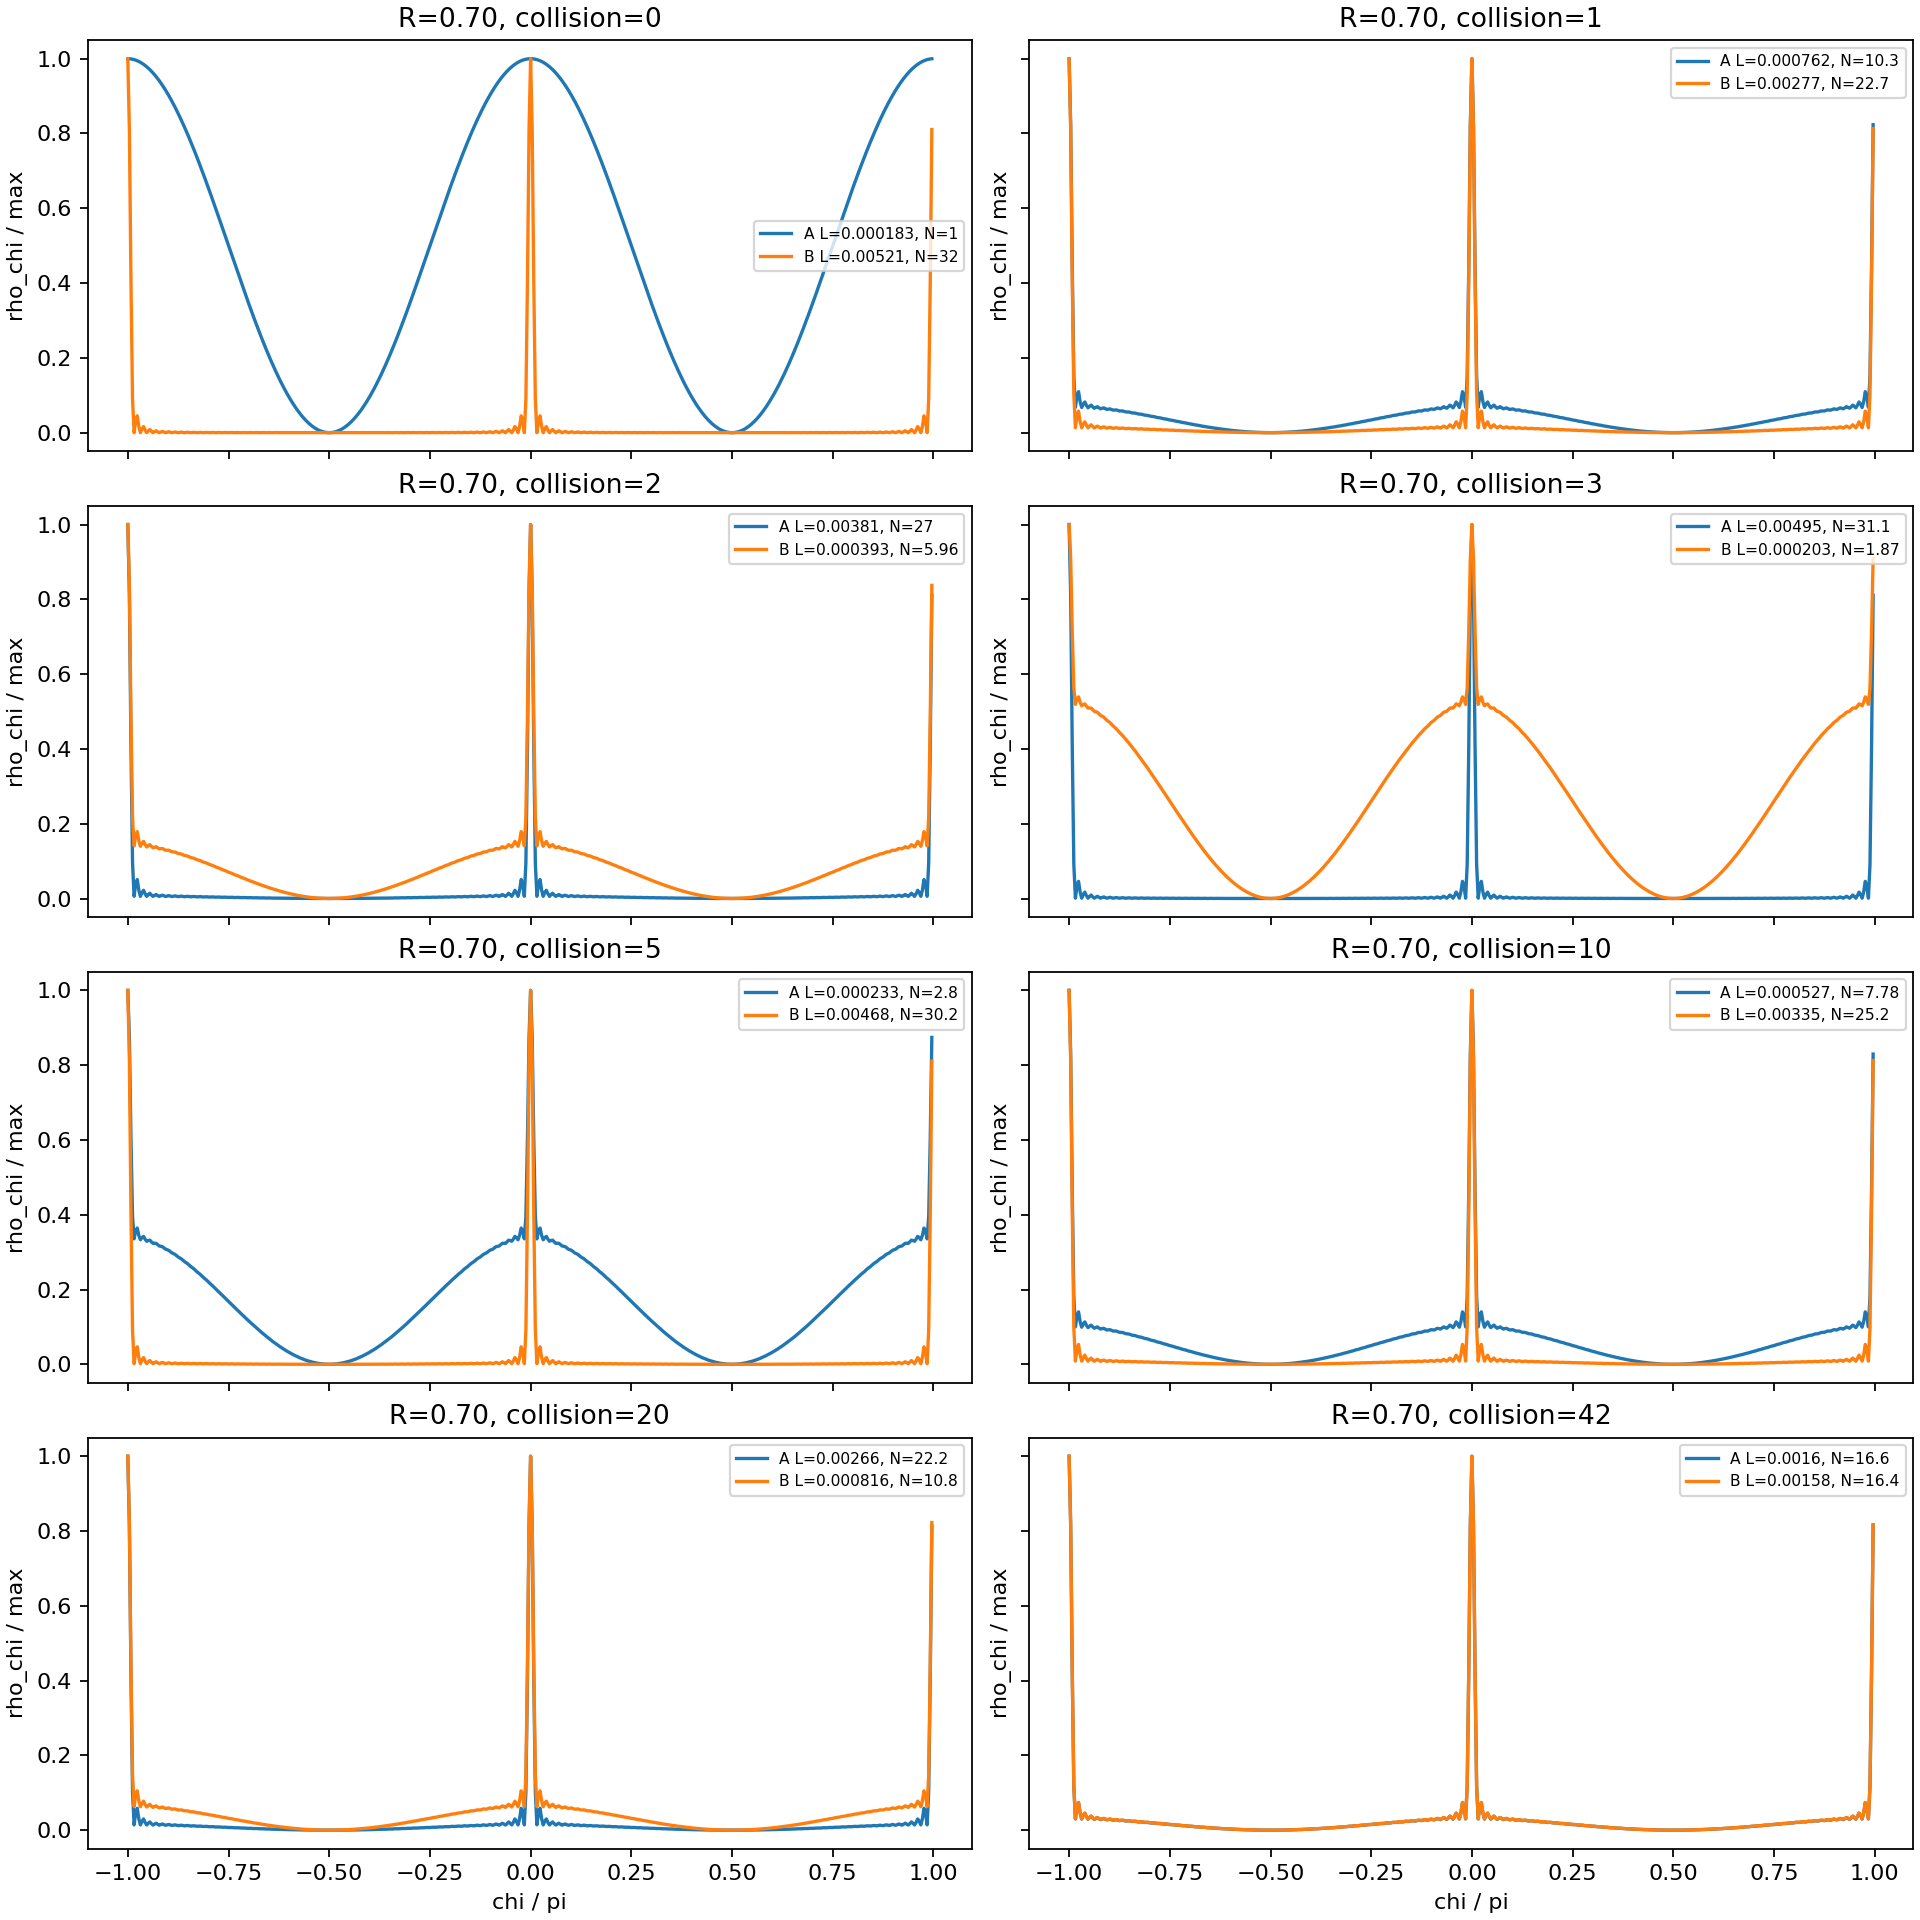
\includegraphics[keepaspectratio,alt={R070 waveform evolution}]{exchange_scattering_matrix_fermionic_localization_transfer_preliminary_result_v1/exchange_scattering_matrix_R070_waveform_evolution_v1.png}}
\caption{R070 waveform evolution}
\end{figure}

\begin{center}\rule{0.5\linewidth}{0.5pt}\end{center}

\subsection{9. Readout-Stop Control}\label{readout-stop-control}

In the readout-on/readout-off control,

\begin{Shaded}
\begin{Highlighting}[]
\NormalTok{observation\_stop\_max\_L\_delta = 0.0}
\end{Highlighting}
\end{Shaded}

was obtained.

Under the readout-on and readout-off conditions, the localization index
\texttt{L} was recorded with the same value.

The recursive map in this experiment contains no dissipative term
depending on readout-wave strength.

\begin{center}\rule{0.5\linewidth}{0.5pt}\end{center}

\subsection{10. Conclusion}\label{conclusion}

The results of this experiment are as follows:

\begin{Shaded}
\begin{Highlighting}[]
\NormalTok{1. The acceleration V2 basis was preserved.}
\NormalTok{2. The odd{-}harmonic bottom was N=1.}
\NormalTok{3. Removing name hair did not change the N=1 bottom.}
\NormalTok{4. At complete transmission R=0, the localization difference was preserved.}
\NormalTok{5. At complete reflection R=1, the localization difference was also preserved.}
\NormalTok{6. At intermediate scattering 0\textless{}R\textless{}1, the localization index L and effective harmonic order N\_eff were recursively exchanged.}
\NormalTok{7. At R=0.70, L and N\_eff of A/B became close at collision 42.}
\NormalTok{8. Within the range of this experiment, periodic exchange, not stationary convergence, was observed.}
\end{Highlighting}
\end{Shaded}

Therefore, localization redistribution in the fermion-like recoil map
appears not at the complete-transmission or complete-reflection
endpoints, but in intermediate scattering with both reflection and
transmission components.

This provides an experimental basis for examining changes in waveform
localization from the internal outgoing channels of the
exchange-interference scattering matrix.

\begin{center}\rule{0.5\linewidth}{0.5pt}\end{center}

\subsection{11. Outputs}\label{outputs}

{\def\LTcaptype{none} % do not increment counter
\begin{longtable}[]{@{}
  >{\raggedright\arraybackslash}p{(\linewidth - 2\tabcolsep) * \real{0.5000}}
  >{\raggedright\arraybackslash}p{(\linewidth - 2\tabcolsep) * \real{0.5000}}@{}}
\toprule\noalign{}
\begin{minipage}[b]{\linewidth}\raggedright
Type
\end{minipage} & \begin{minipage}[b]{\linewidth}\raggedright
File
\end{minipage} \\
\midrule\noalign{}
\endhead
\bottomrule\noalign{}
\endlastfoot
Script &
\texttt{run\_exchange\_scattering\_matrix\_fermionic\_localization\_transfer\_preliminary\_v1.py} \\
JSON &
\texttt{exchange\_scattering\_matrix\_fermionic\_localization\_transfer\_preliminary\_result\_v1/exchange\_scattering\_matrix\_fermionic\_localization\_transfer\_preliminary\_result\_v1.json} \\
CSV &
\texttt{exchange\_scattering\_matrix\_fermionic\_localization\_transfer\_preliminary\_result\_v1/exchange\_scattering\_matrix\_fermionic\_localization\_transfer\_rows\_v1.csv} \\
Validation memo &
\texttt{exchange\_scattering\_matrix\_fermionic\_localization\_exchange\_validation\_memo\_ja.md} \\
Low odd-harmonic bottom figure &
\texttt{exchange\_scattering\_matrix\_fermionic\_localization\_transfer\_preliminary\_result\_v1/exchange\_scattering\_matrix\_low\_n\_bottom\_v1.png} \\
One-sided high-harmonic figure &
\texttt{exchange\_scattering\_matrix\_fermionic\_localization\_transfer\_preliminary\_result\_v1/exchange\_scattering\_matrix\_one\_side\_high\_harmonic\_v1.png} \\
Waveform localization snapshots &
\texttt{exchange\_scattering\_matrix\_fermionic\_localization\_transfer\_preliminary\_result\_v1/exchange\_scattering\_matrix\_waveform\_localization\_snapshots\_v1.png} \\
R=0.70 waveform evolution &
\texttt{exchange\_scattering\_matrix\_fermionic\_localization\_transfer\_preliminary\_result\_v1/exchange\_scattering\_matrix\_R070\_waveform\_evolution\_v1.png} \\
Recursive R sweep figure &
\texttt{exchange\_scattering\_matrix\_fermionic\_localization\_transfer\_preliminary\_result\_v1/exchange\_scattering\_matrix\_recursive\_R\_sweep\_v1.png} \\
Recursive localization figure &
\texttt{exchange\_scattering\_matrix\_fermionic\_localization\_transfer\_preliminary\_result\_v1/exchange\_scattering\_matrix\_recursive\_localization\_transfer\_v1.png} \\
\end{longtable}
}

\begin{center}\rule{0.5\linewidth}{0.5pt}\end{center}

\section{References}\label{references}

\subsection{Self-Citations}\label{self-citations}

\begin{enumerate}
\def\labelenumi{\arabic{enumi}.}
\tightlist
\item
  Noriaki Kihara, ``Basic Axiom System of the Unnamed Equal-Amplitude
  Composite Wave Model v4'', Version DOI:
  \texttt{10.5281/zenodo.21316620}, Concept DOI:
  \texttt{10.5281/zenodo.21315735}, 2026.
\item
  Noriaki Kihara, ``Construction Experiment of Complete Elastic
  Reflection of Fermion-Like Bilocal Waves in a Closed Phase System
  without Assuming Background Space'', Version DOI:
  \texttt{10.5281/zenodo.21332866}, Concept DOI:
  \texttt{10.5281/zenodo.21291018}, 2026.
\item
  Noriaki Kihara, ``Interference Construction of a Complete Reflection
  Map by a Fermion-Like Opposite-Phase Kernel'', Version DOI:
  \texttt{10.5281/zenodo.21332867}, Concept DOI:
  \texttt{10.5281/zenodo.21295479}, 2026.
\item
  Noriaki Kihara, ``Curvature Renormalization and Complete Reflection
  Stability by Curved Closed Stationary Waves'', Version DOI:
  \texttt{10.5281/zenodo.21332874}, Concept DOI:
  \texttt{10.5281/zenodo.21304039}, 2026.
\item
  Noriaki Kihara, ``Construction Experiment of Multigauge Interference
  Readout Conserved Quantities in an ABC Closed Phase System'', Version
  DOI: \texttt{10.5281/zenodo.21332875}, Concept DOI:
  \texttt{10.5281/zenodo.21308049}, 2026.
\item
  Noriaki Kihara, ``Preliminary Summary of Harmonic Readout and c=1 Area
  Sweep in an AB Two-Body Closed Phase System'', Version DOI:
  \texttt{10.5281/zenodo.21332876}, Concept DOI:
  \texttt{10.5281/zenodo.21318696}, 2026.
\end{enumerate}

\subsection{External References}\label{external-references}

\begin{enumerate}
\def\labelenumi{\arabic{enumi}.}
\setcounter{enumi}{6}
\tightlist
\item
  Max Born, ``Zur Quantenmechanik der Stossvorgaenge'',
  \emph{Zeitschrift fuer Physik} 37, 863-867, 1926. DOI:
  \texttt{10.1007/BF01397477}.
\item
  S. Pancharatnam, ``Generalized theory of interference, and its
  applications'', \emph{Proceedings of the Indian Academy of Sciences
  A}, 44, 247-262, 1956.
\item
  B. A. Lippmann and J. Schwinger, ``Variational Principles for
  Scattering Processes. I'', \emph{Physical Review}, 79, 469-480, 1950.
\end{enumerate}

\end{document}
